\documentclass[english,onecolumn]{IEEEtran}
\usepackage[T1]{fontenc}
\usepackage[latin9]{luainputenc}
\usepackage[letterpaper]{geometry}
\geometry{verbose}
\usepackage{amsfonts}
\usepackage{babel}

\usepackage{extarrows}
\usepackage[colorlinks]{hyperref}
\usepackage{listings}
\usepackage{xcolor}
\usepackage[ruled,linesnumbered]{algorithm2e}

\usepackage{amsmath,graphicx}
\usepackage{subfigure} 
\usepackage{cite}
\usepackage{amsthm,amssymb,amsfonts}
\usepackage{textcomp}
\usepackage{bm}
\usepackage{booktabs}
\usepackage{listings}
\definecolor{salmon}{rgb}{1, 0.5020, 0.4471}
\usepackage{xparse}

\usepackage{graphicx} 
\usepackage{amsmath}
\usepackage{extarrows}
\usepackage{listings}
\lstset{language=Matlab}

\NewDocumentCommand{\codeword}{v}{%
\texttt{\textcolor{blue}{#1}}%
}

\lstdefinestyle{mystyle}{
    numberstyle=\color{green},
    numbers=left,                    
    numbersep=5pt,                  
    showspaces=false,                
    showstringspaces=false,
    showtabs=false,                  
    tabsize=2
}

\lstset{style=mystyle}

\providecommand{\U}[1]{\protect\rule{.1in}{.1in}}
\topmargin            -18.0mm
\textheight           226.0mm
\oddsidemargin      -4.0mm
\textwidth            166.0mm
\def\baselinestretch{1.5}


\newcommand{\Rbb}{\mathbb{R}}
\newcommand{\Pb}{\mathbf{P}}
\newcommand{\Ib}{\mathbf{I}}
\newcommand{\vb}{\mathbf{v}}
\newcommand{\Ucal}{\mathcal{U}}
\newcommand{\Wcal}{\mathcal{W}}
\newcommand{\Vcal}{\mathcal{V}}
\newcommand{\Rcal}{\mathcal{R}}
\newcommand{\Ncal}{\mathcal{N}} 


\def\Q{\mathbf{Q}}
\def\A{\mathbf{A}}
\def\R{\mathbf{R}}
\def\I{\mathbf{I}}


\begin{document}

\begin{center}
	\textbf{\LARGE{SI231 - Matrix Computations, Fall 2020-21}}\\
	{\Large Homework Set \#3}\\
	\texttt{Prof. Yue Qiu and Prof. Ziping Zhao}\\
	\texttt{\textbf{Name:}}   	\texttt{ Min Hongqi }  		\hspace{1bp}
	\texttt{\textbf{Major:}}  	\texttt{ IE } 	\\
	\texttt{\textbf{Student No.:}} 	\texttt{ 2020E8018482005}     \hspace{1bp}
	\texttt{\textbf{E-mail:}} 	\texttt{ minhq@sari.ac.cn}
\par\end{center}



\noindent
\rule{\linewidth}{0.4pt}
{\bf {\large Acknowledgements:}}
\begin{enumerate}
    \item Deadline: \textbf{2020-11-01 23:59:00}
    \item Submit your homework at \textbf{Gradescope}. Entry Code: \textbf{MY3XBJ}. 
    Homework \#3 contains two parts, the theoretical part the and the programming part.
    \item About the the theoretical part:
    \begin{enumerate}
            \item[(a)] Submit your homework in \textbf{Homework 3} in gradescope. Make sure that you have correctly select pages for each problem. If not, you probably will get 0 point.
            \item[(b)] Your homework should be uploaded in the \textbf{PDF} format, and the naming format of the file is not specified.
            \item[(c)] You need to use \LaTeX in principle.
            \item[(d)] Use the given template and give your solution in English. Solution in Chinese is not allowed. 
        \end{enumerate}
  \item About the programming part:
  \begin{enumerate}
      \item[(a)] Submit your codes in \textbf{Homework 3 Programming part} in gradescope.
      \item[(b)] Detailed requirements see in Problem 2 and Probelm 3.
  \end{enumerate}
  \item \textbf{No late submission is allowed.}
\end{enumerate}
\rule{\linewidth}{0.4pt}
\newpage 

\section{Understanding projection}
\noindent\textbf{Problem 1}. \textcolor{blue}{(5 points $\times$ 3)}

Suppose that $\Pb\in \Rbb^{n\times n}$ is a projector onto a subspace $\mathcal{U}$ along its orthogonal complement $\mathcal{U}^{\perp}$, then it is called the \textbf{orthogonal projector} onto $\Ucal$.
\begin{enumerate}
    \item Prove that an orthogonal projector must be singular if it is not an identity matrix.
	\item What is the orthogonal projector onto $\mathcal{U}^{\perp}$ along the subspace $\mathcal{U}$?
    \item Let $\Ucal$ and $\Wcal$ be two subspaces of a vector space $\mathcal{V}$, and denote $\Pb_{\Ucal}$ and $\Pb_{\Wcal}$ as the corresponding orthogonal projectors, respectively. Prove that $\Pb_{\Ucal} \Pb_{\Wcal} = 0$ if and only if $\Ucal \perp \Wcal$.
\end{enumerate}

\noindent
\textbf{Solution.}
\begin{enumerate}
\item P is idempotent; i.e., $p^{2}=p$ \\
suppose the eigenvalues of $P$ is $\lambda$ and the associated eigenvector is $\zeta$ \\
then, $P^{2}\zeta=\lambda p \zeta =\lambda^{2}\zeta$\\
there also have $p^{2}\zeta =p \zeta =\lambda\zeta$\\
$\therefore \quad \lambda^{2}=\lambda \quad \Rightarrow \quad \lambda=0 $ or $ 1$\\
if the eigenvalues of $P$ all are $\lambda_{i}=1, \quad i=1,2, \cdots, n$\\
and because $\lambda_{i}=1>0, \quad i=1,2, \cdots, n,$\\
so $P$ is non-singular
matrix. 
$\therefore P^{-1} P^{2}=P^{-1} P \quad \therefore P=I$\\
Otherwise s if there have an eigenvalues of $P$ is 0, then the $P$ singular.
so orthogonal projector must be singular if it is not an identity matrix.


\item
suppose $\alpha_{1}, \alpha_{2}, \cdots, \alpha_{k}$ are the basis of $\mathcal U$ 's column vectors,\\
let $A=\left[\alpha_{1}, \alpha_{2}, \ldots, \alpha_{k}\right]$\\
then the orthogonal projector onto $u$ is
$$
P=A\left(A^{\top} A\right)^{-1} A^{\top}
$$
suppose $\mathcal A=\operatorname{span}\left\{\alpha_{1}, \alpha_{2}, \cdots, \alpha_{k}\right\},$ we have $\mathcal A^{\top}=\mathcal U^{\top}$\\
so the orthogonal projector onto $\mathcal U^{\perp}$ is
$P_{A}^{\perp}=I-A\left(A^{\top} A\right)^{-1} A^{-1}$


\item 
First suppose $P_{U} P_{W}=0 .$ Suppose $w \in W .$ Then
$$
\begin{aligned}
0 &=P_{U} P_{W} w \\
&=P_{U} w
\end{aligned}
$$
Hence $w \in$ $\mathcal N(P_{U})$. so $w \in U^{\perp} .$ Thus $\langle u, w\rangle=0$ for all $u \in U$ completing one direction of the proof.

To prove the other direction, now suppose that $\langle u, w\rangle=0$ for all $u \in U$ and all $w \in W .$ Thus $U \subset W^{\perp}$ and $W \subset U^{\perp} .$ If $w \in W,$ then
$$
\left(P_{U} P_{W}\right)(w)=P_{U}\left(P_{W} w\right)=P_{U} w=0
$$
where the last equality holds because $w \in U^{\perp} .$ If $v \in W^{\perp},$ then
$$
\left(P_{U} P_{W}\right)(v)=P_{U}\left(P_{W} v\right)=P_{U} 0=0
$$
since every element in $V$ can be written as the sum of a vector in $W$ and a vector in $W^{\perp}$, \\
suppose $\nu$ is an arbitrary vector in $V$, and $\nu = w_i + v_j$, \\
then $\left(P_{U} P_{W}\right)\nu = 0$ for every $\nu$ in $V$
\\So that $P_{U} P_{W}=0,$ as desired.



\end{enumerate}







\newpage
\section{Least Square (LS) programming.}
\noindent\textbf{Problem 2}. \textcolor{blue}{(10 points + 10 points + 5 points)}

Write programs to solve the least square problem with specified methods, any programming language is suitable.
$$
\mathbf{x} = \mathop{\arg\min}_{\mathbf{x} \in \Rbb^n} f(\mathbf{x}), \quad f(\mathbf{x}) = ||\mathbf{y}-\mathbf{A}\mathbf{x}||_2^2
$$
where $\mathbf{A} \in \Rbb^{m \times n}$ is a matrix representing the predefined data set with $m$ data samples of $n$ dimensions ($m$=1000, $n$=210), and $\mathbf{y} \in \Rbb^m$ represents the labels. The data samples are provided in the "data.txt" file, and the labels are provided in the "label.txt" file, you are supposed to load the data before solving the problem.

\begin{enumerate}
    \item Solve the LS with gradient decent method.\\
    The gradient descent method for solving problem updates $ {\bf x}$ as
    $$
        {\bf x} = {\bf x} - \gamma \cdot \nabla_{{\bf x}} f(\mathbf{x}),
    $$
    where $\gamma$ is the step size of the gradient decent methods. We suggest that you can set $\gamma=1e-5$.
    \item Solve the LS by the method of normal equation with Cholesky decomposition and forward/backward substitution.
    \item Compare two methods above. 
    \begin{enumerate}
        \item[(a)] Basing on the true running results from the program, count the number of "flops"*;
        \item[(b)] Compare gradient norm and loss $f(\mathbf{x})$ for results $\mathbf{x}=\mathbf{x_{LS}}$ of above two algorithms.
    \end{enumerate}
\end{enumerate}
    \textbf{Notation*:} "flop": one flop means one floating point operation, i.e., one addition, subtraction, multiplication, or division of two floating-point numbers, in this problem each floating points operation $+,-,\times, \div, \sqrt{\cdot}$ counts as one "flop". \\
    \textbf{Hint for gradient decent programming:} 
    \begin{enumerate}
        \item \textbf{Step size selection}: to ensure the convergence of the method, $\gamma$ is supposed to be selected properly (large step size may accelerate the convergence rate but also may lead to instability, A sufficiently small compensation always ensures that the algorithm converges). 
        \item \textbf{Terminal condition}: the gradient decent is an iteration algorithm that need a terminal condition. In this problem, the algorithm can stop when the gradient of the loss function $f(\mathbf{x})$ at current $\mathbf{x}$ is small enough.
    \end{enumerate}
    \noindent\textbf{Remarks: }
   \begin{itemize}
    \item The solution of the two methods should be printed in files named "sol1.txt" and "sol2.txt" and submitted in gradescope.  The format should be same as the input file (210 rows plain text, each rows is a dimension of the final solution).
    \item Make sure that your codes are executable and are consistent with your solutions.
   \end{itemize}
\noindent
\textbf{Solution.}
\begin{enumerate}
\item
\begin{lstlisting}
clear;
clc;
y = load('label.txt');
A = load('data.txt');
x=inv(A'*A)*A'*y;
fid=fopen(['E:\MatlabFile\LS\','sol.txt'],'w');
for m=1:length(x)
    fprintf(fid,'%.16f\r\n',x(m));   
end
f_x=norm(y-A*x)^2
fclose(fid);
x1= Gradient_descent(A,y);
fid=fopen(['E:\MatlabFile\LS\','sol1.txt'],'w');
for i=1:length(x1)
    fprintf(fid,'%.16f\r\n',x1(i));   
end
f_x1=norm(y-A*x1)^2
fclose(fid);
x2=Cholesky_LS(A,y);
fid=fopen(['E:\MatlabFile\LS\','sol2.txt'],'w');
for j=1:length(x2)
    fprintf(fid,'%.16f\r\n',x2(j));   
end
f_x2= norm(y-A*x2)^2
fclose(fid);
\end{lstlisting}

\begin{lstlisting}
function x = Gradient_descent(A,y)
tA = A;
x = ones(size(A,2),1);
k = 0;
while true
    gradient_descent = zeros(size(tA,2),1);
    z = A*x;
    gradient_descent = gradient_descent + 0.00001*A'*(y - z);
    x = x + gradient_descent;
    k = k+1;
    if ( norm(y - A*x)^2 ) <= 2.664261406344091e+04 | k>10000   
        break;
    end
    fprintf('iterator times %d, error %f\n',k,( norm(y - A*x)^2 ));
end
\end{lstlisting}










\item
\begin{lstlisting}
function x = Cholesky_LS(A,y)
C=A'*A;
L=Cholesky_decomposition(C);
y=LU(L,A'*y);
x=LU(L',y);
\end{lstlisting}

\begin{lstlisting}
function L=Cholesky_decomposition(A)
[N,N]=size(A);
X=zeros(N,1);
Y=zeros(N,1);
for i=1:N
    A(i,i)=sqrt(A(i,i)-A(i,1:i-1)*A(i,1:i-1)');
    if A(i,i)==0
        'A is singular, no unique solution';
        break;
    end
    for j=i+1:N
        A(j,i)=(A(j,i)-A(j,1:i-1)*A(i,1:i-1)')/A(i,i);
    end
end
for x=1:N
    for y=1:N
        B(x,y)=A(x,y);    
        if x<y
            B(x,y)=0;
            break;
        end
    end
end
L=B;
\end{lstlisting}

\begin{lstlisting}
function LU_ans = LU(A,b)
N=length(A);
z = zeros(N,1);
LU_ans = zeros(N,1);
L=eye(N);%Let the L matrix be an identity matrix at first
for i=1:N-1
    for j=i+1:N            
            L(j,i)=A(j,i)/A(i,i);
            A(j,:)=A(j,:)-(A(j,i)/A(i,i))*A(i,:);
    end
end
for p=1:1:N
    z(p)=b(p)/L(p,p);
    for q=1:1:p-1
        z(p)=z(p)-z(q)*L(p,q)/L(p,p);        
    end
end
for p_2=N:-1:1
    LU_ans(p_2)=z(p_2)/A(p_2,p_2);
    for q_2=N:-1:p_2+1
        LU_ans(p_2)=LU_ans(p_2)-LU_ans(q_2)*A(p_2,q_2)/A(p_2,p_2);        
    end
end
\end{lstlisting}




\item
\begin{enumerate}
        \item[(a)] Basing on the true running results from the program in the gradient descent method, it iterated 165 times to approximate $x_{LS}$, and in each approximation, if $A$ is $m\times n$ matrix, then it uses $(mn^2+mn+m+3n)$ flops, so it totally uses $165\times (1000\times 210^2+1000\times 210+1000+210\times 3)=44311630$ flops.\\
From the program in the Cholesky decomposition and forward/backward substitution method. In the $Function \ \  L=Cholesky\_decomposition(A)$, it can be computed in $\mathcal{O}\left(n^{3} / 3\right)$, because $n=210$, so it uses $\frac{1}{3} n^{3}+m^{2} n+m \times n+\frac{2}{3} n^{3} \times 2=225645000$ flops.

\item[(b)] In the code script Main.m, I solved that $f(x_1)=2.664261406344088e+04$ and $f(x_2)=2.664261406344087e+04$



    \end{enumerate}
\end{enumerate}

\newpage
\section{Understanding the QR Factorization}
\noindent\textbf{Problem 3 [Understanding the Gram-Schmidt algorithm.]}. \textcolor{blue}{(5 points + 7 points + 6 points + 7 points)}
\begin{enumerate}
	\item 
	Consider the subspace $\mathcal{S}$ spaned by $\{ {\bf a}_1,\ldots, {\bf a}_4\}$, where
	\[
	{\bf a}_1 = \begin{bmatrix} 1 \\ 2 \\ 3 \\ 4\end{bmatrix}\,,\quad 
	{\bf a}_2 =  \begin{bmatrix}2 \\ 3 \\ 4 \\ 5 \end{bmatrix}\,,\quad 
	{\bf a}_3 =  \begin{bmatrix}3 \\ 4 \\5 \\ 6 \end{bmatrix}\,,\quad
	{\bf a}_4 =  \begin{bmatrix}3 \\ 5 \\7 \\ 11 \end{bmatrix}\,.
	\] 
	Use the \textbf{classical} Gram-Schimidt algorithm (See Algorithm \ref{alg:classical_gs}), find a set of orthonormal basis $\{{\bf q}_i\}$ for $\mathcal{S}$ by hand (derivation is expected). \textcolor{black}{
	Do not use decimals in your answers, fraction and $n$-th roots of numbers are accepted.}
	Verify the orthonormality of the found basis.
	\begin{algorithm}[htbp]
 \label{alg:classical_gs}
\SetKwInOut{Input}{Input}\SetKwInOut{Output}{Output}
\caption{Classical Gram-Schmidt algorithm}
\SetAlgoLined
\Input{A collection of linearly independent vectors ${\bf a}_1,\ldots, {\bf a}_n$.}
\textbf{Initilization:} $\widetilde{{\bf q}}_1 = {\bf a}_1, {\bf q}_1 = \widetilde{{\bf q}}_1/\|\widetilde{{\bf q}}_1\|_2$\\
 \For{$i= 2,\ldots, n$}{
  $\widetilde{{\bf q}}_i = {\bf a}_i - \sum_{j=1}^{i-1} ({\bf q}_j^T{\bf a}_i){\bf q}_j$\\
  ${\bf q}_i = \widetilde{{\bf q}}_i/\|\widetilde{{\bf q}}_i\|_2$ 
 }
 \Output{${\bf q}_1,\ldots, {\bf q}_n$}
\end{algorithm}
	\item 
	Orthogonal projection of vector ${\bf a}$ onto a nonzero vector ${\bf b}$ is defined as
	\[
	\text{proj}_\mathbf{b}(\bf a)=\frac{\langle{\bf a},{\bf b}\rangle}{\langle{\bf b},{\bf b}\rangle}{\bf b},
	\]
	where $\langle,\rangle$ denotes the inner product of vectors.
	And for subspace $\mathcal{M}$ with 
	orthonormal basis $\{ {\bf u}_1,\ldots, {\bf u}_k \}$, the orthogonal projector onto subspace $\mathcal{M}$ is given by 
	\[
	{\bf P} = {\bf UU}^T\,,\quad {\bf U} = [{\bf u}_1|\cdots|{\bf u}_k]\,.
	\]
	In the context of \textbf{projection of vector} and \textbf{projection onto subspace} respectively, can you give another two understandings of the classical Gram-Schmidt algorithm?
    %Try to understand Gram-Schmidt algorithm in the context of \textbf{projection onto subspace} and give a new expression of ${\bf q}_k$ based on your understanding.
	%It can b \|\,,\\_2e written as projection of subspace $\bf Pa$ and $\bf P$ is an orthogonal projector, where $\bf P$ is a projection matrix.
	\item Consider the subspace $\mathcal{S}$ spaned by $\{{\bf a}_1, {\bf a}_2, {\bf a}_3\}$,
	\[
	{\bf a}_1 = \begin{bmatrix} 1 \\ \epsilon \\ \epsilon \\ \end{bmatrix}\,,\quad 
	{\bf a}_2 =  \begin{bmatrix}1 \\ \epsilon \\ 0\end{bmatrix}\,,\quad 
	{\bf a}_3 =  \begin{bmatrix}1 \\ 0 \\ \epsilon\end{bmatrix}\,,
	\]
	where $\epsilon$ is a small real number such that $1+k\epsilon^2 =1$ $(k\in\mathbb{N}^+)$. 
	First complete the pseudo algorithm in Algorithm \ref{alg:modified_gs}.
	Then use the \textbf{classical} Gram-Schimidt algorithm and the \textbf{modified} Gram-Schimidt algorithm respectively, find two sets of basis for $\mathcal{S}$ by hand (derivation is expected). Are the two sets of basis the same? If not, which one is the desired orthonormal basis? Report what you have found.
	\begin{algorithm}[htbp]
	\label{alg:modified_gs}
\SetKwInOut{Input}{Input}\SetKwInOut{Output}{Output}
\caption{Modified Gram-Schmidt algorithm}
\SetAlgoLined
\Input{A collection of linearly independent vectors ${\bf a}_1,\ldots, {\bf a}_n$.}
\textbf{Initilization:}  $ \tilde{q}_{1}=a_{1}, \hat{q}_{2}=a_{2} \quad \cdots, \tilde{q}_{n}=a_{n} $    \\
 \For{$i= 1,\ldots, n$}{
  $\widetilde{{\bf q}}_i = \frac{\tilde{{\bf q}_i}}{\|\widetilde{{\bf q}}_i\|^2}$\\
  \For{$j= i+1,\ldots, n$}{
	$\widetilde{{\bf q}}_j=\widetilde{{\bf q}}_j-(\widetilde{{\bf q}}_j{\bf q}_i){\bf q}_i$
}
 }









 \Output{${\bf q}_1,\ldots, {\bf q}_n$}
\end{algorithm}
	\item \textbf{Programming part:}
	In this part, you are required to code both the \textbf{ classical Gram-Schmidt} and \textbf{the modified Gram-Schmidt} algorithms.
	For $\epsilon=1\text{e}-4$ and $\epsilon=1\text{e}-9$ in sub-problem 2), give the outputs of two algorithms and calculate $\|{\bf Q}^T {\bf Q} - {\bf I}\|_{\text{F}}$, where ${\bf Q} = [{\bf q}_1,{\bf q}_2,{\bf q}_3]$.
\end{enumerate}
\noindent\textbf{Remarks: }
\begin{itemize}
    \item Coding languages are restricted, but do not use built-in function such as \codeword{qr}.
    \item When handing in your homework in gradescope, package all your codes into {\sf your\_student\_id+hw3\_code.zip} and upload. In the package, you also need to include a file named {\sf README.txt/md} to clearly identify the function of each file.
     \item Make sure that your codes can run and are consistent with your solutions.
\end{itemize}

\noindent
\textbf{Solution.}
\begin{enumerate}
\item
$$
\tilde{q}_{1}=a_{1}, \quad q_{1}=\frac{\hat{q}_{1}}{\left\|\hat{q}_{1}\right\|_{2}}=\left[\frac{1}{\sqrt{30} }, \frac{2}{\sqrt{30}}, \frac{3}{\sqrt{30}}, \frac{4}{\sqrt{30}}\right]^{\top}
$$
$$
\tilde{q}_{2}=a_{2}-\left(q_{1}^{\top} a_{2}\right) q_{1}=\left[\begin{array}{c}
2 \\
3 \\
4 \\
5
\end{array}\right]-\frac{2+6+12+20}{\sqrt{30}} \cdot\left[\begin{array}{c}
\frac{1}{\sqrt{30}} \\
\frac{2}{\sqrt{30}} \\
\frac{3}{\sqrt{30}} \\
\frac{4}{\sqrt{30}}
\end{array}\right]=\left[\frac{2}{3}, \frac{1}{3}, 0,-\frac{1}{3}\right]
$$
$$
\therefore q_{2}=\frac{\tilde{q}_{2}}{\left\|\tilde{q}_{2}\right\|}=\left[\frac{2}{\sqrt{6}}, \frac{1}{\sqrt{6}}, 0,-\frac{1}{\sqrt{6}}\right]^{\top}
$$

$$
\tilde{q}_{3}=a_{3}-\left(q_{1}^{\top} a_{3}\right) q_{1}-\left(q_{2}^{\top} a_{3}\right) q_{2}=\left[\begin{array}{l}
3 \\
4 \\
5 \\
6
\end{array}\right]-\frac{3+8+15+24}{\sqrt{3} 0}\left[\begin{array}{c}
\frac{1}{\sqrt{30}} \\
\frac{2}{\sqrt{30}} \\
\frac{3}{\sqrt{30}} \\
\frac{4}{\sqrt{30}}
\end{array}\right]-\frac{6+4-6}{\sqrt{6}}\left[\begin{array}{c}
\frac{2}{\sqrt{6}} \\
\frac{1}{\sqrt{6}} \\
0 \\
-\frac{1}{\sqrt{6}}
\end{array}\right]=\left[\begin{array}{c}
0 \\
0 \\
0 \\
0
\end{array}\right]
$$

$$
\begin{array}{l}
q_{3}=\tilde{q}_{3}=\left[\begin{array}{llll}
0 & 0 & 0 & 0
\end{array}\right]^{\top} \\
\tilde{q}_{4}=a_{4}-\left(q_{1}^{\top} a_{4}\right) q_{1}-\left(q_{2}^{\top} a_{4}\right) q_{2}-\left(q_{3}^{\top} a_{4}\right) q_{3}= \left[\begin{array}{c}3 \\ 5 \\ 7 \\ 11\end{array}\right]-\frac{3+10+21+44}{\sqrt{30}}\left[\begin{array}{c}\frac{1}{\sqrt{30}} \\ \frac{1}{\sqrt{30}} \\ \frac{1}{\sqrt{30}} \\ \frac{1}{\sqrt{30}}\end{array}\right]=\left[\begin{array}{c}\frac{2}{5} \\ -\frac{1}{5} \\ -\frac{4}{5} \\ \frac{3}{5}\end{array}\right]\\
\therefore q_{4}=\frac{\tilde{q}_{4}}{\left\|\tilde{q}_{4}\right\|}=\left[\frac{2}{\sqrt{30}},-\frac{1}{\sqrt{30}},-\frac{4}{\sqrt{30}}, \frac{3}{\sqrt{30}}\right]^{\top}
\end{array}
$$

\item In the context of projection of vector, we can have a geometrical understanding of the classical Gram-Schmidt algorithm:
\\Given a basis $\alpha_{1}, \alpha_{2}, \ldots, \alpha_{n}$, convert it to another orthonormal basis $\beta_{1}, \beta_{2}, \ldots, \beta_{n}$ so that the two bases are equivalent.
\\$\beta_{1}=\alpha_{1}$
\\$\beta_{2}=\alpha_{2}-\frac{\left(\alpha_{2}, \beta_{1}\right)}{\left(\beta_{1}, \beta_{1}\right)} \beta_{1}$
$\ldots$
\\$\beta_{n}=\alpha_{n}-\frac{\left(\alpha_{n}, \beta_{1}\right)}{\left(\beta_{1}, \beta_{1}\right)} \beta_{1}-\frac{\left(\alpha_{n}, \beta_{2}\right)}{\left(\beta_{2}, \beta_{2}\right)} \beta_{2}-\ldots-\frac{\left(\alpha_{n}, \beta_{n-1}\right)}{\left(\beta_{n-1}, \beta_{n-1}\right)} \beta_{n-1}$
\\First of all,Orthogonal projection of vector ${\bf \alpha}$ onto a nonzero vector ${\bf\beta}$ is defined as
	$\text{proj}_\mathbf{\beta}(\bf \alpha)=\frac{\langle{\bf \alpha},{\bf \beta}\rangle}{\langle{\bf \beta},{\bf \beta}\rangle}{\bf \beta}$, 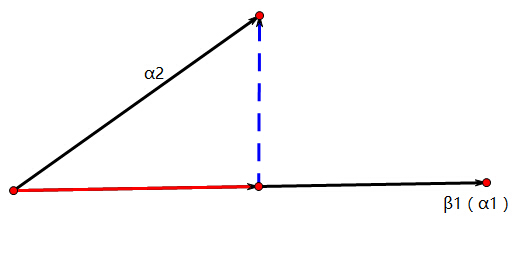
\includegraphics[width=2.77in,height=1.75in]{1.jpg} 
\\The red vector is the projection part, so the blue vector is $\alpha_{2}-\frac{\left(\alpha_{2}, \beta_{1}\right)}{\left(\beta_{1}, \beta_{1}\right)} \beta$, that corresponds to Gram-Schmidt algorithm's $\beta_2$. So $\beta_2$ is perpendicular to $\beta_1$
\\When the number of vectors is 3, the geometric interpretation of the corresponding three-dimensional space is shown in the figure:
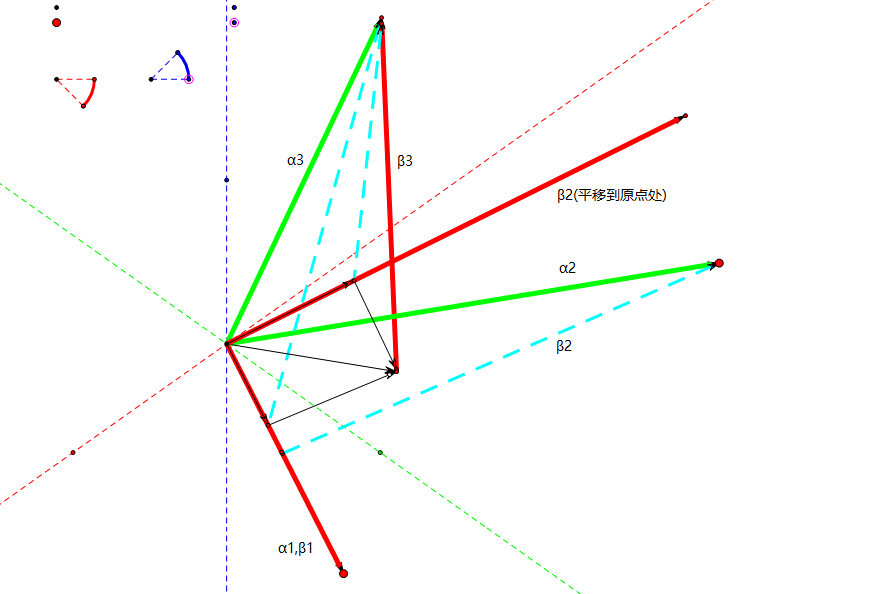
\includegraphics[width=4.77in,height=3.75in]{2.jpg} 
\\The green vector is the original base $\alpha_{i}$, $\alpha_{1}$ is red because $\alpha_{1}$ is also $\beta_{1}$, I'm going to shift  $\beta_{2}$ to the origin, then the orthogonal projection of  $\alpha_{3}$ onto XoY plane is $\alpha_{3}-\frac{\left(\alpha_{3}, \beta_{1}\right)}{\left(\beta_{1}, \beta_{1}\right)} \beta_{1}-\frac{\left(\alpha_{3}, \beta_{2}\right)}{\left(\beta_{2}, \beta_{2}\right)} \beta_{2}$
\\We can see that $\beta_{1}\ \beta_{2}\  \beta_{3}$ are orthoogonal, it can also be extended to Euclidean space above three dimensions.

\item  Use the \textbf{classical} Gram-Schimidt algorithm: \\
Suppose $\varepsilon$ is positive,\\
$\tilde{q}_{1}=a_{1} \quad q_{1}=\frac{\hat{q}_{1}}{\left\|q_{1}\right\|}=\left[\frac{1}{\sqrt{1+2 \varepsilon^{2}}}, \frac{\varepsilon}{\sqrt{1+2 \varepsilon}^{2}}, \frac{\varepsilon}{\sqrt{1+2 \varepsilon^{2}}}\right]^{\top}=\left[\begin{array}{lll}1 & \varepsilon & \varepsilon\end{array}\right]^{\top}$
\\ \\
$\tilde{q}_{2}=a_{2}-\left(q_{1}^{\top} a_{2}\right) q_{1}=\left[\begin{array}{c}1 \\ \varepsilon \\ 0\end{array}\right]-\left(1+\varepsilon^{2}\right)\left[\begin{array}{c}1 \\ \varepsilon \\ \varepsilon\end{array}\right]=\left[\begin{array}{c}-\varepsilon^{2} \\ -\varepsilon^{3} \\ -\varepsilon-\varepsilon^{3}\end{array}\right]=\left[\begin{array}{c}0 \\ 0 \\ -\varepsilon\end{array}\right],\left\|\tilde{q}_{i}\right\|=\varepsilon$
\\$q_{2}=\frac{\tilde{q}_{2}}{\| \tilde{q}_{n}||}=\left[\begin{array}{c}0 \\ 0 \\ -1\end{array}\right]$
\\$\tilde{q}_{3}=a_{3}-\left(q_{1}^{\top} a_{3}\right) q_{1}-\left(q_{2}^{\top} u_{3}\right) q_{2}=\left[\begin{array}{c}1 \\ 0 \\ \varepsilon\end{array}\right]-\left(1+\varepsilon^{2}\right)\left[\begin{array}{c}1 \\ \varepsilon \\ \varepsilon\end{array}\right]-(-\varepsilon)\left[\begin{array}{c}0 \\ 0 \\ 1\end{array}\right]=\left[\begin{array}{c}0 \\ -\varepsilon \\ -\varepsilon\end{array}\right]$
\\ \\$q_{3}=\frac{\tilde{q}_{3}}{\left\|\tilde{q}_{3}\right\|}=\left[\begin{array}{ccc}0 & -\frac{1}{\sqrt{2}} & -\frac{1}{\sqrt{2}}\end{array}\right]^{\top}$\\\\
Use the \textbf{modified} Gram-Schimidt algorithm: \\
$\tilde{q}_{1}=a_{1} \quad, \quad q_{1}=\frac{\hat{q}_{1}}{\left\|\hat{q}_{1}\right\|}=\left[\frac{1}{\sqrt{1+2 \varepsilon^{2}}}, \frac{\varepsilon}{\sqrt{1+2 \varepsilon^{2}}}, \frac{\varepsilon}{\sqrt{1+2 \varepsilon^{2}}}\right]^{\top}=\left[\begin{array}{lll}1 & \varepsilon & \varepsilon\end{array}\right]^{\top}$\\ \\
$\tilde{q}_{2}=a_{2}-\left(q_{1}^{T} a_{2}\right) q_{1}=\left[\begin{array}{c}1 \\ \varepsilon \\ 0\end{array}\right]-\left(1+\varepsilon^{2}\right)\left[\begin{array}{c}1 \\ \varepsilon \\ \varepsilon\end{array}\right]=\left[\begin{array}{c}-\varepsilon^{2} \\ -\varepsilon^{3} \\ -\varepsilon-\varepsilon^{3}\end{array}\right]=\left[\begin{array}{c}0 \\ 0 \\ -\varepsilon\end{array}\right]$\\
\\$q_{2}=\frac{\tilde{q}_{2}}{\left\|\hat{q}_{2}\right\|}=\left[\begin{array}{lll}0 & 0 & -1\end{array}\right]^{\top}$
\\\\$a_{3}^{(1)}=a_{3}-\left(q_{1}^{\top} a_{3}\right) q_{1}=\left[\begin{array}{l}1 \\ 0 \\ \varepsilon\end{array}\right]-\left(1+\varepsilon^{2}\right)\left[\begin{array}{l}1 \\ \varepsilon \\ \varepsilon\end{array}\right]=\left[\begin{array}{c}0 \\ -\varepsilon \\ 0\end{array}\right]$\\
\\\\$a_{3}^{(2)}=a_{3}^{(1)}-\left(q_{2}^{\top} a_{3}^{(1)}\right) q_{2}=\left[\begin{array}{c}0 \\ -\varepsilon \\ 0\end{array}\right]-0=\left[\begin{array}{c}0 \\ -\varepsilon \\ 0\end{array}\right]$
$\therefore q_{3}=\frac{a_{3}^{(2)}}{\left\|a_{3}^{(2)}\right\|}=\left[\begin{array}{c}0 \\ -1 \\ 0\end{array}\right]$\\
so the two sets of basis are not same,the one that use the modified Gram-Schimidt algorithm is the desired orthonormal basis.In the classical Gram-Schimidt algorithm's answer, we get $q_{2}^{\top} q_{3}=\frac{1}{\sqrt{2}} \neq 0$, so $q_{2}$ and $q_{3}$ are not orthogonal. But in the classical Gram-Schimidt algorithm's answer, we get $q_{1}^{\top} q_{2}=-\varepsilon^{2}=0 ,\quad q_{1}^{\top} q_{3}=-\varepsilon ,\quad q_{2}^{\top} q_{3}=0$, so $q_{1}, q_{1}, q_{1}$ are orthogonal except a slight error $\varepsilon$.

\item
\begin{lstlisting}
clear all;clc;
% a1=[1;2;3;4];
% a2=[2;3;4;5];
% a3=[3;4;5;6];
% a4=[3;5;7;11];
% A=[a1 a2 a3 a4];
e=1e-4;
a1=[1;e;e];
a2=[1;e;0];
a3=[1;0;e];
A=[a1 a2 a3];
Q_classical= Classical_GS(A)
normF_1=norm(Q_classical,'fro')
Q_modified= Modified_GS(A)
normF_2=norm(Q_modified,'fro')
e=1e-9;
Q_classical_1= Classical_GS(A)
normF_11=norm(Q_classical_1,'fro')
Q_modified_2= Modified_GS(A)
normF_2=norm(Q_modified_2,'fro')
\end{lstlisting}
The output is:
\begin{lstlisting}
Q_classical =             %e=1e-4
   0.999999990000000   0.000099999998782   0.000099999999892
   0.000099999999000   0.000000010000000  -0.999999995000000
   0.000099999999000  -0.999999995000000   0.000000002820298
normF_1 =
     3.988504106090590e-09
Q_modified =
   0.999999990000000   0.000099999998782   0.000099999999782
   0.000099999999000   0.000000010000000  -0.999999995000000
   0.000099999999000  -0.999999995000000   0.000000000000000
normF_2 =
     5.640596652684282e-13
Q_classical_1 =          %e=1e-9
   0.999999990000000   0.000099999998782   0.000099999999892
   0.000099999999000   0.000000010000000  -0.999999995000000
   0.000099999999000  -0.999999995000000   0.000000002820298
normF_11 =
     3.988504106090590e-09
Q_modified_2 =
   0.999999990000000   0.000099999998782   0.000099999999782
   0.000099999999000   0.000000010000000  -0.999999995000000
   0.000099999999000  -0.999999995000000   0.000000000000000
normF_2 =
     5.640596652684282e-13
\end{lstlisting}
\end{enumerate}



\newpage
\section{SOLVING LS VIA QR FACTORIZATION AND NORMAL EQUATION}
\noindent\textbf{Problem 4 [Understanding the influence of the condition number to the solution.]}. \textcolor{blue}{(4 points + 5 points + 4 points + 4 points + 3 points points) }

Consider such two LS problems:
\begin{align}
    &\min_{{\bf x}\in\mathbb{R}^n} \|{\bf Ax - b}\|_2^2 \label{axb}\\
    &\min_{{\bf x}\in\mathbb{R}^n} \|{\bf A}{\bf x} - ({\bf b}+\delta{\bf b })\|_2^2 \nonumber%\label{withnoise}
\end{align}
with ${\bf A}\in \mathbb{R}^{m\times n}$. For ${\bf b} = \begin{bmatrix}
    1 & 3/2 & 3 & 6
    \end{bmatrix}^T$
    and 
    $\delta{\bf b} = \begin{bmatrix}
    1/10 & 0 & 0 & 0
    \end{bmatrix}^T$,

\begin{enumerate}
    \item Computing solution to the problem (\ref{axb})
    via QR decomposition when \[{\bf A}=
    \begin{bmatrix}
    1 & 2 & 3\\
    2 & 3 & 5\\
    3 & 4 & 7\\
    4 & 5 & 11
    \end{bmatrix}. \]
    
    \item For a full-rank matrix ${\bf A}$, consider the equation ${\bf Ax=b}$, after adding some noise $\delta{\bf b}$ to {\bf b}, we have ${\bf A}({\bf x}+\delta{\bf x}) = {\bf b}+\delta{\bf b}$, 
    and then proof
    $$ \frac{1}{\|{\bf A}\| \|{\bf A}^{\dagger}\|} \frac{\|\delta {\bf b}\|}{\|{\bf b}\|}
    \leq \frac{\|\delta {\bf x}\|}{\|{\bf x}\|} \leq
    \|{\bf A}\| \|{\bf A}^{\dagger}\|\frac{\|\delta {\bf b}\|}{\|{\bf b}\|}, $$
    and give it a plain interpretation.
    
    \item Computing the solutions to the two LS problems via the normal equation $ {\bf A}^T{\bf A}{\bf x}_{LS} = {\bf A}^T {\bf b} $ when \[{\bf A}=\begin{bmatrix}
    1 & 2 & 2\\
    2 & 2 & 2\\
    3 & 3 & 3\\
    1 & 1 & 0
    \end{bmatrix}.  \]
    
    \item Computing the solutions to the two LS problems via the normal equation $ {\bf A}^T{\bf A}{\bf x}_{LS} = {\bf A}^T {\bf b} $ when \[ {\bf A} = \begin{bmatrix}
    1 & 1 & 1\\
    1 & 2 & 4\\
    1 & 3 & 9\\
    1 & 4 & 16
    \end{bmatrix}. \]
    
    \item 
    Compare the 2-norm condition number $\|{\bf A}\|\| {\bf A}^{\dagger}\|$ for ${\bf A}$ in 3) and 4) and the influence on the solution to problem (\ref{axb}) 
    resulted by the additional noise $\delta{\bf b}$.
    
    \noindent{\bf Hint:} Show the influence on the solution  by $\frac{\|\delta {\bf x}\|}{\|{\bf x}\|}$.
\end{enumerate}




\noindent{\bf Remarks:} You can use MATLAB for some matrix computations (deviation is expected) in 3), 4), 5).
Do not use decimals in your answers, fraction and $n$-th roots of numbers are accepted.

\noindent
\textbf{Solution.}
\begin{enumerate}
\item 
let $r_{i i}=\left\|\tilde{\mathbf{q}}_{i}\right\|_{2}, r_{j i}=\mathbf{q}_{j}^{T} \mathbf{a}_{i}$ for $j=1, \ldots, i-1$
we see that $\mathbf{a}_{i}=\sum_{j=1}^{i} r_{j i} \mathbf{q}_{i}$ for all $i,$ or, equivalently,
$\left[\begin{array}{llll}\mathbf{a}_{1} & \mathbf{a}_{2} & \ldots & \mathbf{a}_{n}\end{array}\right]=\left[\begin{array}{llll}\mathbf{q}_{1} & \mathbf{q}_{2} & \ldots & \mathbf{q}_{n}\end{array}\right]\left[\begin{array}{llll}r_{11} & r_{12} & \cdots & r_{1 n} \\ & r_{22} & \cdots & r_{2 n} \\ & & \ddots & \vdots \\ & & & r_{n n}\end{array}\right]$\\
use the solution above, we can get \\\\
$\tilde{q}_{1}=\left[\begin{array}{l}1 \\ 2 \\ 3 \\ 4\end{array}\right], q_{1}=\left[\begin{array}{c}\frac{1}{\sqrt{30}} \\ \frac{2}{\sqrt{30}} \\ \frac{3}{\sqrt{30}} \\ \frac{4}{\sqrt{30}}\end{array}\right], \quad \tilde{q}_{2}=\left[\begin{array}{c}\frac{2}{3} \\ \frac{1}{3} \\ 0 \\ -\frac{1}{3}\end{array}\right], q_{2}=\left[\begin{array}{c}\frac{2}{\sqrt{b}} \\ \frac{1}{\sqrt{6}} \\ 0 \\ -\frac{1}{\sqrt{6}}\end{array}\right]$
$\tilde{q}_{3}=\left[\begin{array}{c}\frac{2}{5} \\ -\frac{1}{5} \\ -\frac{4}{5} \\ \frac{3}{5}\end{array}\right]$
$q_{3}=\left[\begin{array}{c}\frac{2}{\sqrt{30}} \\ -\frac{1}{\sqrt{30}} \\ -\frac{4}{\sqrt{30}} \\ \frac{3}{\sqrt{30}}\end{array}\right]$\\ 
\\\\So $ \quad Q_{1}=\left[\begin{array}{lll}q_{1} & q_{2} & q_{3}\end{array}\right]=\left[\begin{array}{ccc}\frac{1}{\sqrt{30}} & \frac{2}{\sqrt{6}} & \frac{2}{\sqrt{30}} \\ \frac{2}{\sqrt{30}} & \frac{1}{\sqrt{6}} & -\frac{1}{\sqrt{30}} \\ \frac{3}{\sqrt{30}} & 0 & -\frac{4}{\sqrt{30}} \\ \frac{4}{\sqrt{30}} & -\frac{1}{\sqrt{6}} & \frac{3}{\sqrt{30}}\end{array}\right]$, \quad
$R_{1}=\left[\begin{array}{cccc}r_{11} & r_{12} & \cdots & r_{1 n} \\ r_{21} & r_{22} & \cdots & r_{2 n} \\ & & \ddots & \vdots \\ & & & r_{n n}\end{array}\right]=\left[\begin{array}{ccc}\sqrt{3}_{0} & \frac{{40}}{\sqrt{30}} & \frac{78}{\sqrt{30}} \\ 0 & \frac{2}{\sqrt{6}} & 0 \\ 0 & 0 & \frac{\sqrt{30}}{5}\end{array}\right]$\\\\
$min\{\|A x-b\|_{2}^{2}\}=min\{\left\|Q_{1}^{\top} b-R_{1} x\right\|_{2}^{2}\} \quad\left(\right.$ because $\left.Q_{2}= 0 \right)$
\\
$z=Q_{1}^{T} b=\left[\begin{array}{cccc}\frac{1}{\sqrt{30}} & \frac{2}{\sqrt{30}} & \frac{3}{\sqrt{30}} & \frac{4}{\sqrt{30}} \\ \frac{2}{\sqrt{6}} & \frac{1}{\sqrt{6}} & 0 & -\frac{1}{\sqrt{6}} \\ \frac{2}{\sqrt{20}} & -\frac{1}{\sqrt{30}} & -\frac{4}{\sqrt{30}} & \frac{3}{\sqrt{30}}\end{array}\right] \quad\left[\begin{array}{c}1 \\ \frac{3}{2} \\ 3 \\ 6\end{array}\right]$
$=\left[\frac{37}{\sqrt{30}}-\frac{5}{2 \sqrt{6}}, \frac{13}{2 \sqrt{30}}\right]^{\top}$\\
then solve $\quad R_{1} x=z$\\
$x=R_{1}^{-1} z=\left[\begin{array}{ccc}\frac{1}{12} & -\frac{5}{4} & \frac{13}{12}\end{array}\right]^{\top}$

\item 
$\because A(x+\delta x)=b+\delta b$\\
$\therefore x(1+\delta)=A^{\dagger}(1+\delta) b$\\
$\therefore \delta x=\delta A^{\dagger} b$\\
$\therefore\|\delta x\|=\left\|\delta A^{\dagger} b\right\| \leqslant\left\|A^{\dagger}\right\|\|\delta b\|$\\
$\therefore A x=b$\\
$\therefore \|b\|=\| A x\|\leqslant\| A\|\| x \|$\\
$\frac{1}{\|x\|} \leqslant \frac{\|A\|}{\|b\|}$\\
multiply $(*)$ and $(* *),$ we can get
$\frac{\|\delta x\|}{\|x\|} \leqslant\|A\|\left\|A^{\dagger}\right\| \frac{\|\delta b\|}{\|b\|}$\\
$\because \delta A x=\delta b$\\
$\therefore\|\delta b\| \leqslant\|\delta A x\| \leqslant\|A\|\|\delta x\|$\\
$\therefore \frac{\|\delta b\|}{\|A\|} \leqslant\|\delta x\|$\\
$\because x=A^{\dagger} b$\\
$\therefore\|x\| \leqslant\left\|A^{\dagger}\right\|\|b\|$\\
$\therefore \frac{1}{\left\|A^{\dagger}\right\|\|b\|} \leqslant \frac{1}{\|x\|}$\\
multiply (1) and (2), we can get
$\frac{1}{\|\mathbf{A}\|\left\|\mathbf{A}^{+}\right\|} \frac{\|\delta \mathbf{b}\|}{\|\mathbf{b}\|} \leqslant \frac{\|\delta \mathbf{x}\|}{\|\mathbf{x}\|}$\\
so $\frac{1}{\|\mathbf{A}\|\left\|\mathbf{A}^{+}\right\|} \frac{\|\delta \mathbf{b}\|}{\|\mathbf{b}\|} \leq \frac{\|\delta \mathbf{x}\|}{\|\mathbf{x}\|} \leq\|\mathbf{A}\|\left\|\mathbf{A}^{\dagger}\right\| \frac{\|\delta \mathbf{b}\|}{\|\mathbf{b}\|}$\\

\item
$x_{1}=\left(A^{\top} A\right)^{-1} A^{\top} b=\left[\begin{array}{lll}\frac{11}{13} & \frac{67}{13} & -\frac{66}{13}\end{array}\right]^{\top}$\\\\
$x_{2}=\left(A^{\top} A\right)^{-1} A^{\top}(b+\delta b)=\left[\frac{97}{130} \frac{683}{130}-\frac{66}{13}\right]^{\top}$\\

\item
$x_{1}=\left(A^{\top} A\right)^{-1} A^{\top} b=\left[\frac{15}{8}-\frac{59}{40} \quad \frac{5}{8}\right]^{\top}$\\\\
$x_{2}=\left(A^{\top} A\right)^{-1} A^{\top}(b+\delta b)=\left[\frac{21}{10}-\frac{163}{100} \frac{13}{20}\right]^{\top}$\\

\item
$A^{\dagger}=\left(A^{\top} A\right)^{-1} A^{\top}$\\
For problem $(3): \quad\|A\|=6.982 \quad\left\|A^{\dagger}\right\|=1.908$\\
$So, \quad\|A\|\left\|A^{\dagger}\right\|=13.325$\\
$\delta x=x_{2}-x_{1}=\left[-\frac{1}{10}, \frac{1}{10}, 0\right]^{\top}$\\
$\frac{\|\delta x\|}{\|x\|}=\frac{\left\|x_{2}-x_{1}\right\|}{\left\|x_{1}\right\|}=\frac{125}{6438}=0.0194$




For problem $(4): \quad\|A\|=19.621 \quad\left\|A^{\dagger}\right\|=3.756$\\
$So, \quad\|A\|\left\|A^{\dagger}\right\|=73.694$\\
$\delta x=x_{2}-x_{1}=\left[\frac{9}{40},-\frac{31}{200}, \frac{1}{40}\right]^{\top}$\\
$\frac{\|\delta x\|}{\|x\|}=\frac{\left\|x_{2}-x_{1}\right\|}{\left\|x_{1}\right\|}=\frac{1231}{11065}=0.1113$

\end{enumerate}


\newpage
\section{Underdetermined System}

\noindent\textbf{Problem 5 [Solving Underdetermined System by QR]}. \textcolor{blue}{(10 points + 5 points)}

Consider the following underdetermined system ${\bf Ax}={\bf b}$ with ${\bf A}\in \mathbb{R}^{m\times n}$ and $m<n$. Let 
    \[
    {\bf A}=
    \begin{bmatrix}
         1&2&2&0\\
         0&-2&2&1\\
         2&5&6&1
    \end{bmatrix}\,,
    {\bf b}=
    \begin{bmatrix}
        b_1\\b_2\\b_3
    \end{bmatrix}\,,
    \]
\begin{enumerate}
    \item Use Householder reflection to give the full QR decomposition of tall ${\bf A}^T$, i.e., $\A^T= \Q\R$ with $\Q$ being a square matrix with orthonormal columns.
    \item Give one possible solution via QR decomposition of $\A^T$, write down your solution using $\bf{b}$.
\end{enumerate}
\noindent
\textbf{Solution.}
\begin{enumerate}
\item $A^{T}=\left[\begin{array}{ccc}1 & 0 & 2 \\ 2 & -2 & 5 \\ 2 & 2 & 6 \\ 0 & 1 & 1\end{array}\right]=\left[\alpha_{1},\alpha_{2}, \alpha_{3}\right]$\\
$v_{1}=a_{1}-\left\|\alpha_{1}\right\| e_{1}=\left[\begin{array}{cccc}-2 & 2 & 2 & 0\end{array}\right]^{\top}$\\
$H_{1}=I-\frac{2}{\left\|v_{1}\right\|_{2}^{2}} v_{1} v_{1}^{\top}$\\
Then $A^{(1)}=H_{1} A^{\top}=\left[\begin{array}{rrr}3 & 0 & 8 \\ 0 & -2 & -1 \\ 0 & 2 & 0 \\ 0 & 1 & 1\end{array}\right]$\\
$u_{2}=\left[\begin{array}{ccc}-2 & 2 & 1\end{array}\right]^{1}$\\
$\therefore v_{2}=u_{2}-\left\|u_{2}\right\| e_{1}=\left[\begin{array}{ccc}-5 & 2 & 1\end{array}\right]^{\top}$\\
$\therefore \hat{H}_{2}=I-\frac{2}{\left\|v_{2}\right\|_{2}^{2}} v_{2} v_{2}^{\top}=\left[\begin{array}{rrr}-\frac{2}{3} & \frac{2}{3} & \frac{1}{3} \\ \frac{2}{3} & \frac{11}{15} & -\frac{2}{15} \\ \frac{1}{3} & -\frac{2}{15} & \frac{14}{15}\end{array}\right]$\\
$H_{2}=\left[\begin{array}{ll}1 & 0 \\ 0 & \tilde{H}_{2}\end{array}\right]$\\
$A^{(2)}=H_{2} A^{(1)}=H_{2} H_{1} A^{\top}=\left[\begin{array}{ccc}3 & 0 & 8 \\ 0 & 3 & 1 \\ 0 & 0 & -\frac{4}{5} \\ 0 & 0 & \frac{3}{5}\end{array}\right]$\\
$u_{3}=\left[-\frac{4}{5} \quad \frac{3}{5}\right]^{\top}$\\
$\therefore v_{3}=u_{3}-\left\|u_{3}\right\| e_{1}=\left[-\frac{9}{5} \quad \frac{3}{5}\right]^{\top}$\\
$\therefore \tilde{H}_{3}=I-\frac{2}{\left\|V_{3}\right\|_{2}^{2}} v_{3} v_{3}^{\top}=\left[\begin{array}{cc}-\frac{4}{5} & \frac{3}{5} \\ \frac{3}{5} & \frac{4}{5}\end{array}\right]$\\
$\therefore H_{3}=\left[\begin{array}{cc}I_{2} & 0 \\ 0 & \tilde{H}_{3}\end{array}\right]$\\
$then \quad A^{(3)}=H_{3} A^{(2)}=H_{3} H_{2} H_{1} A^{T}=\left[\begin{array}{lll}3 & 0 & 8 \\ 0 & 3 & 1 \\ 0 & 0 & 1 \\ 0 & 0 & 0\end{array}\right]=R$\\
$Q = H_1H_2H_3 =\left[\begin{array}{rrrr}\frac{1}{3} & 0 & -\frac{2}{3} & \frac{2}{3} \\ \frac{2}{3} & -\frac{2}{3} & \frac{1}{3} & 0 \\ \frac{2}{3} & \frac{2}{3} & 0 & -\frac{1}{3} \\ 0 & \frac{1}{3} & \frac{2}{3} & \frac{2}{3}\end{array}\right]$\\

\item
For $\mathbf{A} \in \mathbb{R}^{m \times n}$ with $m<n$ and $\operatorname{rank}(\mathbf{A})=m,$ we have
$$
\mathbf{A}^{T}=\mathbf{Q} \mathbf{R}=\left[\begin{array}{ll}
\mathbf{Q}_{1} & \mathbf{Q}_{2}
\end{array}\right]\left[\begin{array}{c}
\mathbf{R}_{1} \\
\mathbf{0}
\end{array}\right]=\mathbf{Q}_{1} \mathbf{R}_{1}+\mathbf{Q}_{2} \mathbf{0}
$$
- note
$$
\mathbf{A} \mathbf{x}=\mathbf{R}_{1}^{T} \mathbf{Q}_{1}^{T} \mathbf{x}+\mathbf{0}^{T} \mathbf{Q}_{2}^{T} \mathbf{x}=\mathbf{b}
$$
which indicates
$$
\mathbf{Q}_{1}^{T} \mathbf{x}=\mathbf{R}_{1}^{-T} \mathbf{b}
$$
and $\mathrm{Q}_{2}^{T} \mathrm{x}$ can be anything, which we set to be $\mathrm{d}$. Then we have
$$
\left[\begin{array}{c}
\mathbf{Q}_{1}^{T} \mathbf{x} \\
\mathbf{Q}_{2}^{T} \mathbf{x}
\end{array}\right]=\mathbf{Q}^{T} \mathbf{x}=\left[\begin{array}{c}
\mathbf{R}_{1}^{-T} \mathbf{b} \\
\mathbf{d}
\end{array}\right]
$$
- the solution is
$$
\mathbf{x}=\mathbf{Q}\left[\begin{array}{c}
\mathbf{R}_{1}^{-T} \mathbf{b} \\
\mathbf{d}
\end{array}\right]=\mathbf{Q}_{1} \mathbf{R}_{1}^{-T} \mathbf{b}+\mathbf{Q}_{2} \mathbf{d}
$$
where to get the minimum norm solution, we can set $\mathrm{d}=0$.
so, $$
\mathbf{x}=\mathbf{Q}\left[\begin{array}{c}
\mathbf{R}_{1}^{-T} \mathbf{b} \\
\mathbf{d}
\end{array}\right]=\mathbf{Q}_{1} \mathbf{R}_{1}^{-T} \mathbf{b}
$$
$\begin{aligned} \because & Q_{1}=\left[\begin{array}{rrr}\frac{1}{3} & 0 & -\frac{2}{3} \\ \frac{2}{3} & -\frac{2}{3} & \frac{1}{3} \\ \frac{2}{3} & \frac{2}{3} & 0 \\ 0 & \frac{1}{3} & \frac{2}{3}\end{array}\right], \quad R_{1}=\left[\begin{array}{ccc}3 & 0 & 8 \\ 0 & 3 & 1 \\ 0 & 0 & 1\end{array}\right] \\ \therefore & x=\left[\begin{array}{ccc}\frac{17}{9} & \frac{2}{9} & -\frac{2}{3} \\ -\frac{2}{3} & -\frac{1}{3} & \frac{1}{3} \\ \frac{2}{9} & \frac{2}{9} & 0 \\ -\frac{16}{9} & -\frac{1}{9} & \frac{2}{3}\end{array}\right]\left[\begin{array}{c}b_{1} \\ b_{2} \\ b_{3}\end{array}\right] =\left[\begin{array}{l}
\frac{17}{9} b_{1}+\frac{2}{9} b_{2}-\frac{2}{3} b_{3} \\
-\frac{2}{3} b_{1}-\frac{1}{3} b_{2}+\frac{1}{3} b_{3} \\
\frac{2}{9} b_{1}+\frac{2}{9} b_{2} \\
-\frac{16}{9} b_{1}-\frac{1}{9} b_{2}+\frac{2}{3} b_{3}
\end{array}\right] \end{aligned}$





\end{enumerate}

\newpage
\section{Solving LS via Projection}
\noindent\textbf{Problem 6}. \textcolor{blue}{(Bonus question, 6 points + 4 points)}

Consider the Least Square (LS) problem:
\begin{equation}
    \label{eq:LS_problem}
    \min_{\mathbf{x}\in\mathbb{R}^n}\|\mathbf{A}\mathbf{x}-\mathbf{y}\|_2^2
\end{equation}
where $\mathbf{A}\in\mathbb{R}^{m\times n}$ ($m>n$) may not be full rank. Denote 
\begin{equation*}
    X_{\mathrm{LS}}=\left\{\mathbf{x}\in\mathbb{R}^n| \mathbf{A}^T\mathbf{A}\mathbf{x}=\mathbf{A}^T\mathbf{y}\right\}
\end{equation*}
as the set of all solutions to (\ref{eq:LS_problem}), and 
\begin{equation*}
    \mathbf{x}_{\mathrm{LS}}=\mathbf{A}^\dagger \mathbf{y}
\end{equation*}
where $\mathbf{A}^\dagger\in\mathbb{R}^{n\times m}$ is the \emph{pseudo inverse of $\mathbf{A}$} satisfies the following properties:
\begin{enumerate}
    \item $\mathbf{A}\mathbf{A}^\dagger\mathbf{A}=\mathbf{A}$.
    \item $\mathbf{A}^\dagger\mathbf{A}\mathbf{A}^\dagger=\mathbf{A}^\dagger$.
    \item $(\mathbf{A}\mathbf{A}^\dagger)^T=\mathbf{A}\mathbf{A}^\dagger$.
    \item $(\mathbf{A}^\dagger\mathbf{A})^T=\mathbf{A}^\dagger\mathbf{A}$.
\end{enumerate}

Answer the following questions:
\begin{enumerate}
    \item Prove that $\mathbf{x}_{\mathrm{LS}}$ is a solution to (\ref{eq:LS_problem}) and is of minimum $2$-norm in $X_{\mathrm{LS}}$, that is
    \begin{equation*}
        \mathbf{x}_{\mathrm{LS}}=\min\{\|\mathbf{x}\|_2^2|\  \mathbf{x}\in X_{\mathrm{LS}}\}\,.
    \end{equation*}
    \textbf{Hint}. Notice that the orthogonal projection onto $\mathcal{N}(A)$ is given by
    \begin{equation*}
        \mathbf{\Pi}_{\mathcal{N}(A)}=\mathbf{I}-\mathbf{A}^\dagger\mathbf{A}
    \end{equation*}
    
    \item Prove that $X_{\mathrm{LS}}=\{\mathbf{x}_{\mathrm{LS}}\}$ if and only if $\mathrm{rank}({\bf A})=n$.
\end{enumerate}

\noindent
\textbf{Solution.}
\begin{enumerate}
\item
$\because X_{L S}=\left\{x \in \mathbb{R}^{n} \mid A^{\top} A x=A^{\top} y\right\}$\\
$x_{L S}=A^{\dagger} y \in \mathbb{R}^{n}$\\
$A^{\top} A x_{L S}=A^{\top} A A^{\dagger} y=A^{\top}\left(A A^{\dagger}\right)^{\top} y=A^{\top}\left(A^{\dagger}\right)^{\top} A^{\top} y=\left(A^{\dagger} A\right)^{\top} A^{\top} y=\left(A A^{\dagger} A\right)^{\top} y=A y$\\
$\therefore x_{L S} \in X_{L S}$\\
$\therefore x_{L S}$ is a solution to (2)

Suppose $\hat{x}$ is a solution of $A^{\top} A x=A^{\top} y$\\
$i \cdot e \cdot \hat{x} \in X_{L S}$
then $\left\{\begin{array}{l}A^{\top} A \hat{x}=A^{\top} y \quad \Rightarrow \quad A^{\top} A\left(\hat{x}-x_{L S}\right)=0 \\ A^{\top} A x_{L S}=A^{\top} y\end{array}\right.$\\
$\therefore \hat{x}-x_{L S} \in \mathcal{N}\left(A^{\top} A\right)=N(A)$\\
$\begin{aligned} \because \quad \Pi_{N(A)} x_{L S} &=\left(I-A^{\dagger} A\right) x_{L S}=x_{L S}-A^{\dagger} A x_{L S}=x_{L S}-A^{\dagger} A A^{\dagger} y \\ &=x_{L S}-A^{\dagger} y=0 \end{aligned}$\\
$\therefore \quad x_{L S} \in R(A)$\\
$\therefore \quad x_{L S} \perp (\hat{x}-x_{L S})$\\
$\therefore\|\hat{x}\|^{2}=\left\|\left(\hat{x}-x_{L S}\right)+x_{L S}\right\|^{2}=\left\|\hat{x}-x_{L S}\right\|^{2}+\left\|x_{L S}\right\|^{2} \geqslant\left\|x_{L S}\right\|^{2}$


So $\mathrm{x}_{\mathrm{LS}}=\arg \min _{\mathrm{x} \in X_{\mathrm{LS}}}\|\mathrm{x}\|_{2}$

\item
If $X_{\mathrm{LS}}=\left\{\mathrm{x}_{\mathrm{LS}}\right\}$\\
Then $\mathrm{A}^{T} \mathrm{A} X=\mathrm{A}^{T} y$ has a unique solution. \\
$\therefore \mathrm{A}^{\mathrm{T}} \mathrm{A}$ is column full rank.\\
$\because \mathcal{R}(\mathbf{A})=\mathcal{R}\left(\mathbf{A}^{\mathbf{T}} \mathbf{A}\right)$, then $(\mathbf{A})=n$\\
If rank $(\mathbf{A})=n, then \ \mathbf{A}^{\mathbf{T}} \mathbf{A}$ is invertible, the solution of equation $\mathbf{A}^{T} \mathbf{A} \mathbf x=\mathbf{A}^{T} y$ is unique, it means that $X_{\mathrm{LS}}=\left\{\mathrm{x}_{\mathrm{LS}}\right\}$\\
Above all, $X_{\mathrm{LS}}=\left\{\mathrm{x}_{\mathrm{LS}}\right\}$ if and only if $\operatorname{rank}(\mathrm{A})=n$


\end{enumerate}

\end{document}



